\section{Overview of the \sysname{} Framework}
\label{sec:overview}

\subsection{The \sysname{} Building Blocks}
\label{sec:overview:arch}

\sysname{} is a port of \graphene{} \libos{} to \sgx{},
to secure native Linux application in \sgx{} enclaves.
The portability of \graphene{} is discribed in \S\ref{sec:graphene:impl}.
\sysname{} uses the non-partitioned model
to secure applications,
thus only minimal effort is required for developers
to port applications to \sysname{}.

%\graphene{} \libos{} originally runs on Linux hosts, but with the platform
%adaption layer (PAL) ported to other platform,
%\graphene{} can run Linux applications on other hosts such as
%Windows, BSD or OSX.
%\graphene{} supports up to 139 most commonly used Linux system calls
%(300 in total),
%providing reasonable Linux platform compliance.

The building blocks are shown as figure~\ref{fig:gsgx:arch}.
\sysname{} is partitioned into two parts:
an untrusted \pal{} to initialize the enclave and provide the untrusted interface;
and the trusted \libos{} including the host ABI, {\tt libLinux}, and core {\tt libc} libraries.
Except the host ABI is statically loaded in the enclave since the start up,
other components of \sysname{} in the enclave are dynamically loaded,
as needed. 
%For each binary loaded by \sysname{}, \sysname{} bootstraps the enclave
%from an untrusted platform adaption layer (PAL) that defines
%a narrowed untrusted interface.
%To speed up initialization, the untrusted PAL starts the enclave
%with an statically linked library image ({\tt graphene.so}).
%The image includes
%\graphene{} host ABI,
%\libos{} ({\tt libLinux}, implementing Linux personality),
%and basic libraries of GNU library C
%({\tt libc}, {\tt libpthread} and {\tt ld}, the runtime loader).
%The \sysname{} library image then loads the unmodified applications
%and libraries into the enclave.
After the \libos{} is laoded in the enclave,
the \libos{} will load the application and its supporting libraries,
and call their entry functions.
The \libos{} will handle all the system calls redirected from the applications,
whereas it may access host resource through the host ABI calls,
which are redirected to the untrusted interface
to interact with the untrusted host. 

\begin{figure}[t!]
\centering
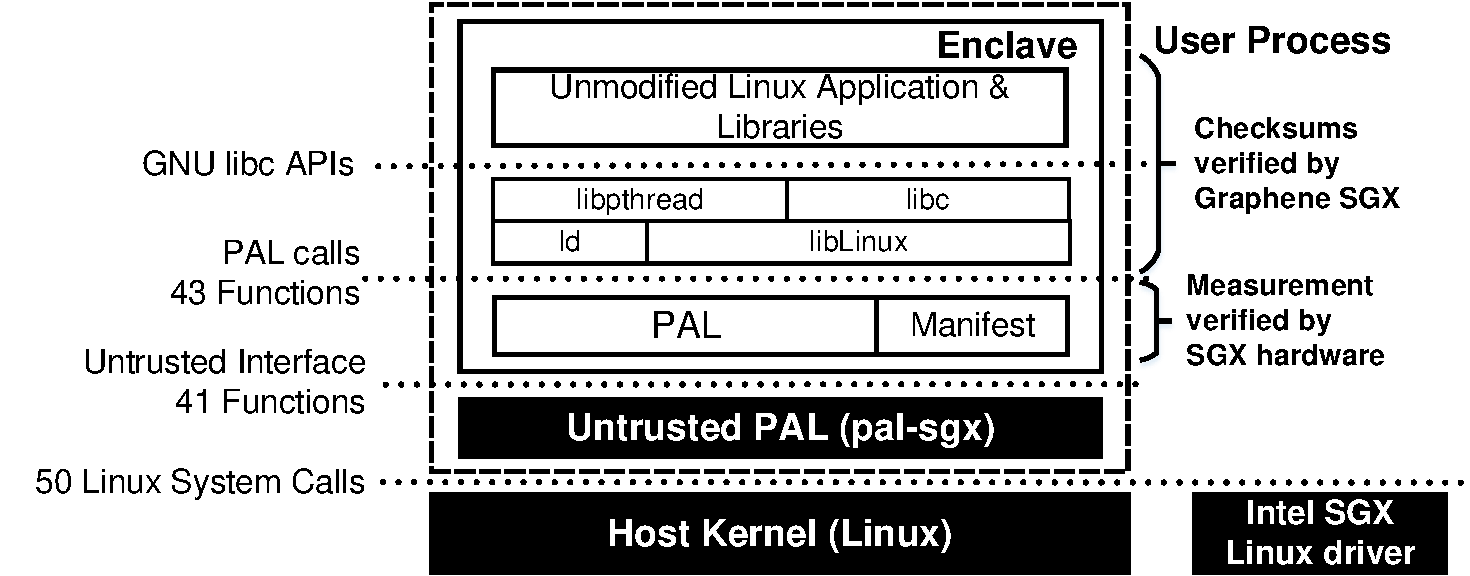
\includegraphics[width=3.8in]{graphene-sgx/figures/architecture.pdf}
\footnotesize
\caption[\sysname{}: building blocks.]
{The \sysname{} building blocks.
Green (light) boxes are trusted components trusted,
and red (dark) boxes are untrusted.
\sysname{} is statically linked with {\tt libLinux},
the \libos{} binary, and basic libraries of GNU library C.
To build up the trust, the \sysname{} image along with
a manifest and application measurements
are verified by \sgx{} during bootstrap. Applications and other libraries
are verified by \sysname{}. The enclave interacts with the host kernel,
through untrusted PAL, on a narrowed untrusted interfaces with xx functions.}
\label{fig:gsgx:arch}
\end{figure}

\paragraph{Integrity Guarantee for Applications.}
A key requirement of the non-partitioned usage model is to guarantee the integrity of the secured applications.
Because the applications are dynamically loaded by the \libos{}
{\em after} the enclave starts up,
the CPUs cannot verify the integrity of loaded application binaries.
An alternative is to place all application binaries in an encrypted virtual disk,
which can be decrypted using a securely provisioned key~\citep{baumann14haven}.

\sysname{} guarantees the integrity of applications
by signing each supporting binaries or generating checksums for the binaries.
For each secured application, the \sysname{} signing tool will generate
a manifest and a correspondent signature.
A manifest will contain the attributes of the enclave and \libos{},
and the checksums of the supporting binaries.
The manifest will be loaded in the enclave before the enclave starts,
and verified by the hardware as part of the enclave measurement.
The signatures of checksums of the supporting binaries
are verified by \sysname{} before loading from the untrusted host.

By verify the integrity of applications individually,
we decouple the deployment and verification of the application binaries;
users may simply deploy the manifest and the signature to the untrusted host,
and all the binaries, including the \libos{}, can be loaded from the local file system.

\paragraph{Untrusted Interface.}
The untrusted interface is defined as Table~\ref{tab:gsgx:interface}.
\sysname{} draws the untrusted interface right above the calling
of the host APIs (Linux system calls) in \pal{}.
Most code inherited from the \graphene{} Linux \pal{} stays in
the enclave, to keep the states secure.
Because the host is not trusted,
\sysname{} is built upon the assumption that the untrusted interface
can be exploited to
pass malicious arguments, or return incorrect results.
For example, {\tt file\_open} may return a file descriptor that points
to a wrong file, or {\tt map\_untrusted} may return an address in the enclave. 
Beside checking for malicious returned results,
\sysname{} must actively check the behavior of the host.

For instance, if the secured application opens a stream for IO,
\sysname{} must guarantee either the stream is protected cryptographically,
or assume that nothing is safely read or written.
In addition, \sysname{} does not include {\tt file\_sync} in the untrusted interface,
because it does not trust the host to faithfully flush any stream.
With a robustly designed untrusted interface,
the worst scenario a malicious host can cause is {\em denial-of-the-service}.

%The Untrusted interface of an enclave is the API that communicates the enclave
%and the untrusted host, with both entries and exits of the enclave.
%Note that for hardware an enclave only has exactly one entry and exit,
%to which execution jumps
%using {\tt EENTER} and {\tt EEXIT} instructions.
%The untrusted interface is simply a callback table that redirects execution
%afterward (similar to system calls).

\begin{table}[t!]
\centering
\footnotesize
\begin{tabular}{lc>{\palign[\tt]{l}}p{4.5in}}
\hline
\addlinespace
Classes & \# & {\normalfont\bf Untrusted Interface Functions} \\
\addlinespace
\hline
Entries / Exits & 3 & 
start\_enclave
exit\_enclave
start\_thread
\\
\hline
Memory & 2 &
map\_untrusted
unmap\_untrusted
\\
\hline
Scheduling & 4 &
sleep
schedule
futex
gettime
\\
\hline
Cloning & 2 &
clone\_thread
clone\_process
\\
\hline
Files & 8 &
file\_open
file\_mkdir
file\_rename
file\_delete
file\_truncate
file\_write
file\_read
file\_readdir
\\
\hline
Sockets & 8 &
sock\_listen
sock\_accept
sock\_connect
socketpair
sock\_send
sock\_receive
sock\_shutdown
sock\_setopt
\\
\hline
File Descriptors & 3 &
fd\_close
fd\_size
fds\_poll
\\
\hline
Misc & 3 &
print\_debug
load\_gdb
cpuid
\\
\hline
\end{tabular}

\caption[\sysname{}: the untrusted interface.]
{Untrusted interface of \sysname{}, consisting of \interfacenum{} functions in total.
Most of the interface is derived from the host system call footprint of
\graphene{} \libos{}. Enclave must not trust the hosts to
always return right responses or faithfully perform operations.}
\label{tab:gsgx:interface}
\end{table}

%\paragraph{The Signing Tool.}
%Each enclave launched in \sgx{} requires a signature, signed by the developers' private key.
%The signature structure ({\tt SIGSTRUCT}) contains
%the enclave attributes, product ID, the enclave measurement,
%and RSA-based signature of the structure.
%\sysname{} maintains enclave signatures on a per-binary basis.
%Unlike \haven{}, we extend the enclave's measurement to
%cover all binaries loaded in the enclave, not just the \libos{} itself.
%To keep the application binaries being dynamically loaded,
%the measurement of these binary files are stored as
%{\bf application checksums}, verified by \sysname{} at loading.
%With the application checksums being measured in enclaves,
%different binaries loaded with different library dependencies
%will naturally yield different measurements,
%easily differentiating the attestations generated by processors.

%Although \haven{} only includes the shielding module
%in the enclave measurements,
%it can still differentiate applications by forcing different digests
%on the same shielding module.
%The trick is to inject an unique ID for each application,
%into the module binary.
%We argue that \sysname{} uses a more straightforward model, with no need to
%maintain the uniqueness of any IDs.
%
%
%
%
%
%
%
%However, carefully engineering the untrusted interface is simply not enough
%to secure the enclave.
%We must not rely on the applications to always
%sanitize IO or encrypt the streams,
%especially if the applications are formally assumed to run on trusted host.
%\sysname{} requires clients to provide {\bf manifests} to state
%the policy of applications while accessing the untrusted interface.
%The manifests are measured, so their integrity can be attested by processors.
%For example, all streams opened must be either encrypted or signed,
%unless the manifest explicitly states ones as unimportant
%(e.g., debug streams).
%Another type of policies can be used for authenticate other ends of RPC streams
%based on the measurements of target enclaves.
%These policies are used to decentralize the trust in multi-process applications,
%that we will discuss in length in section~\ref{sec:multiproc}.

\paragraph{Threat model.}
When an application is loaded by \sysname{}, it ought to be trusted by
certain remote entities
for provisioning confidential information or
accepting the enclave's computation results.
The trusted application code in the enclave includes both
{\bf static} and {\bf dynamic} parts.
The host ABI, library OS, and basic GNU lib C are loaded statically
at the enclave launching time,
with their integrity verified by the processor.
Otherwise, any code that is dynamically loaded, or generated at runtime
(e.g., by just-in-time compilation),
must be secured by \sysname{} or other trusted parts.

For multi-process applications, each process created by \sysname{}
will be isolated in its own enclave.
By default, no trust is required between the processes,
unless the {\bf manifest} specifies any policy
that allows sharing multi-process abstractions.
For example, a parent process can decide to pass output to a child process
through a secured pipe,
but the parent process does not have to trust the child, assuming
the parent will sanitize any information passed to the child.
For processes that have the same security level,
clients can also put them into a mutually trusted group,
where all processes are allowed to share any abstractions.

Besides the enclaves where applications are loaded,
an architectural enclave called {\tt aesm} on each platform that supports \sgx{}
must be trusted by all enclave.
{\tt aesm} is a secured service signed by \intel{} for generating
valid enclave tokens.
The {\tt aesm} binary is part of the \sgx{} SDK,
and signed using an \intel{} internal key, thus cannot be
tampered by any third party.
Otherwise, any other parts of the platform that launches the enclave
must not be trusted, including the host kernel,
\sgx{} kernel driver, and most parts of the hardware except the processor.

\paragraph{Remote attestation.}
For enclaves, the only way to be securely provisioned by another entity
is by attestation.
\sgx{} provides a signed proof of the enclave measurement,
which can be verified by other entities as long as their platforms
also support \sgx{}.
In \haven{} model, the same shielding module cannot have different applications
securely provisioned, because their enclave measurements will simply
appear no difference.
Because \sysname{} includes the applications into enclave measurements,
\sgx{} can generate attestation that differentiates the loaded applications.

\paragraph{Side-channel attacks}
Since enclaves are launched on untrusted hosts, it is hard to prevent
enclaves from becoming vulnerable to side-channel attacks.
Potentially attackers may exploit timing channels to expose confidential
information in the enclave, and current \sgx{} technology has no defense
against these attacks.

Recent works~\citep{xu15controlledchannel} suggest a stronger
side-channel attacks to applications in enclaves,
called {\em controlled channel attacks}.
Controlled channel attacks rely on the fact that an enclave must cooperate
with the host OS for page management,
the OS can manipulate paging to reinforce the side channels
for exposing more secrets.
Currently there is no defense against this type of attacks, except minimizing
the side channels by rearranging code and data in enclave pages.

Both side-channel attacks and Controlled channel attacks
are common problems in all solutions based on \sgx{},
including \haven{}. In this paper, we consider solving these attacks as
out of the scope to our work.

